\documentclass[12pt]{beamer}
\usepackage{amsmath, amssymb, amsfonts, amsthm}
\usepackage{fontspec}
\usepackage{tikz}
\usepackage{graphicx}

\usetheme{Rochester}
\usecolortheme{clean}

\newtheorem{thm}{Theorem}

\title{Final Presentation}
\author{Group 15 (Isaac Bankier, Quinn Bruckmann, Jay Jones, Ngai Chun Fu, Oliver Lambert , Zara Bandukwala)}
\date{22 05 2022}

\beamertemplatenavigationsymbolsempty

\AtBeginSection[]{
  \begin{frame}
    \vfill
    \centering
    \begin{beamercolorbox}[sep=8pt,center,shadow=true,rounded=true]{title}
      \usebeamerfont{title}\insertsectionhead\par%
    \end{beamercolorbox}
    \vfill
  \end{frame}
}

\begin{document}
\begin{frame}
  \maketitle
\end{frame}

\begin{frame}[plain]
  \frametitle{Buisness Case}
  FlyDreamAir is a major airline that covers a wide range of routes throughout the world, has a large fleet of aircrafts and has a large network of travel agencies and customers across the world. But we found that our company has a lack of IT software system that provide better customer experience and increase customer loyalty.\\
  To modernise Fly Dream Air we must build a system that allows customers to continue booking services in the old way while simultaneously allowing customers to move to a new self serve system.
\end{frame}

\begin{frame}[plain]
  \frametitle{Resource Management}
  \begin{columns}
    \begin{column}{0.5\textwidth}
      \textbf{Documentation Devlopment}
      \begin{itemize}
      \item Zara Bandukwala​
      \item Oliver Lambert​
      \item Ngai Chun Fu
      \end{itemize}
    \end{column}
    \begin{column}{0.5\textwidth}
      \textbf{Project Manager}
      \begin{itemize}
      \item Quinn Bruckmann
      \end{itemize}
      \textbf{Software Development}
      \begin{itemize}
      \item Isaac Bankier
      \end{itemize}
    \end{column}
  \end{columns}
\end{frame}

\begin{frame}[plain]
  \frametitle{Scope}
  \begin{columns}
    \begin{column}{0.5\textwidth}
      \textbf{Customers}
      \begin{itemize}
      \item Book Flights
      \item Manage flight reservations
      \item Purchase in flight services
      \end{itemize}
    \end{column}
    \begin{column}{0.5\textwidth}
      \textbf{Employees}
      \begin{itemize}
      \item View available Seats
      \item View Seats and Services booked by a Particular Customer
      \item Perform actions on behalf of users
      \end{itemize}
    \end{column}
  \end{columns}
\end{frame}

\begin{frame}[plain]
  \frametitle{Wbs}
  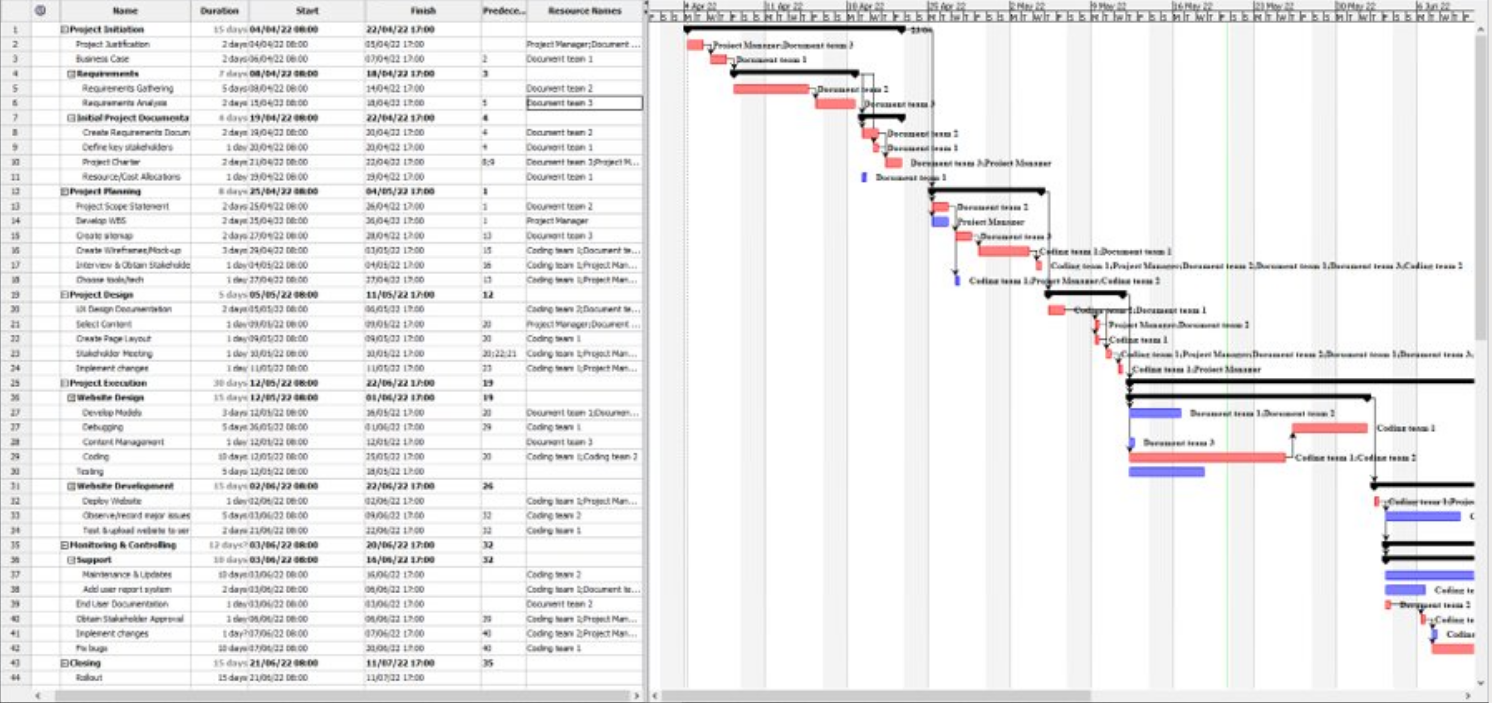
\includegraphics[width=\textwidth]{wbs}
\end{frame}

\begin{frame}[plain]
  \frametitle{Costs}
  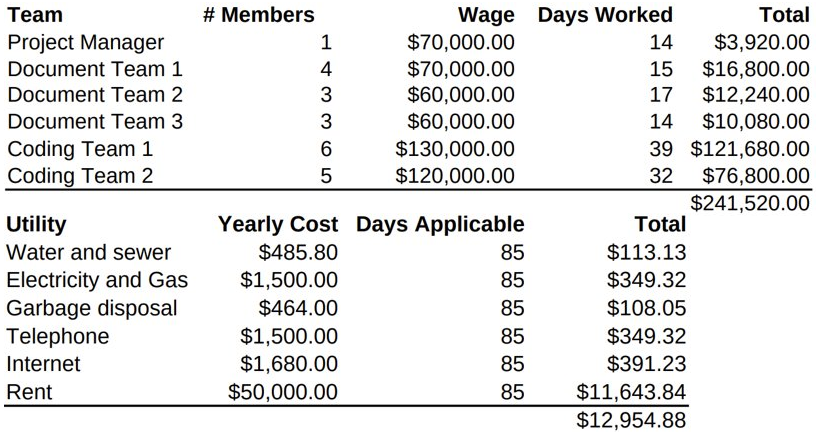
\includegraphics[width=\textwidth]{costs}
\end{frame}

\begin{frame}[plain]
  \frametitle{Cost Benefit Analysis}
  \begin{enumerate}
  \item The total cost is ~\$250,000
  \item The new system reduces barriers to booking with Fly Dream Air
  \item The new system allows better comparisons to be made between airlines
  \item The costs of taking bookings no longer raise with the amount of bookings taken  
  \end{enumerate}
\end{frame}

\begin{frame}[plain]
  \frametitle{Risks}
  We identified 13 risks that could threaten the completion of the project. More than half of these occured. These had the biggest impact on us:
  \begin{enumerate}
  \item Inadequet information on the project requirements
  \item Issues with communication of decisions
  \item Slippage in Schedule
  \end{enumerate}
\end{frame}

\begin{frame}[plain]
  \frametitle{Demo}
  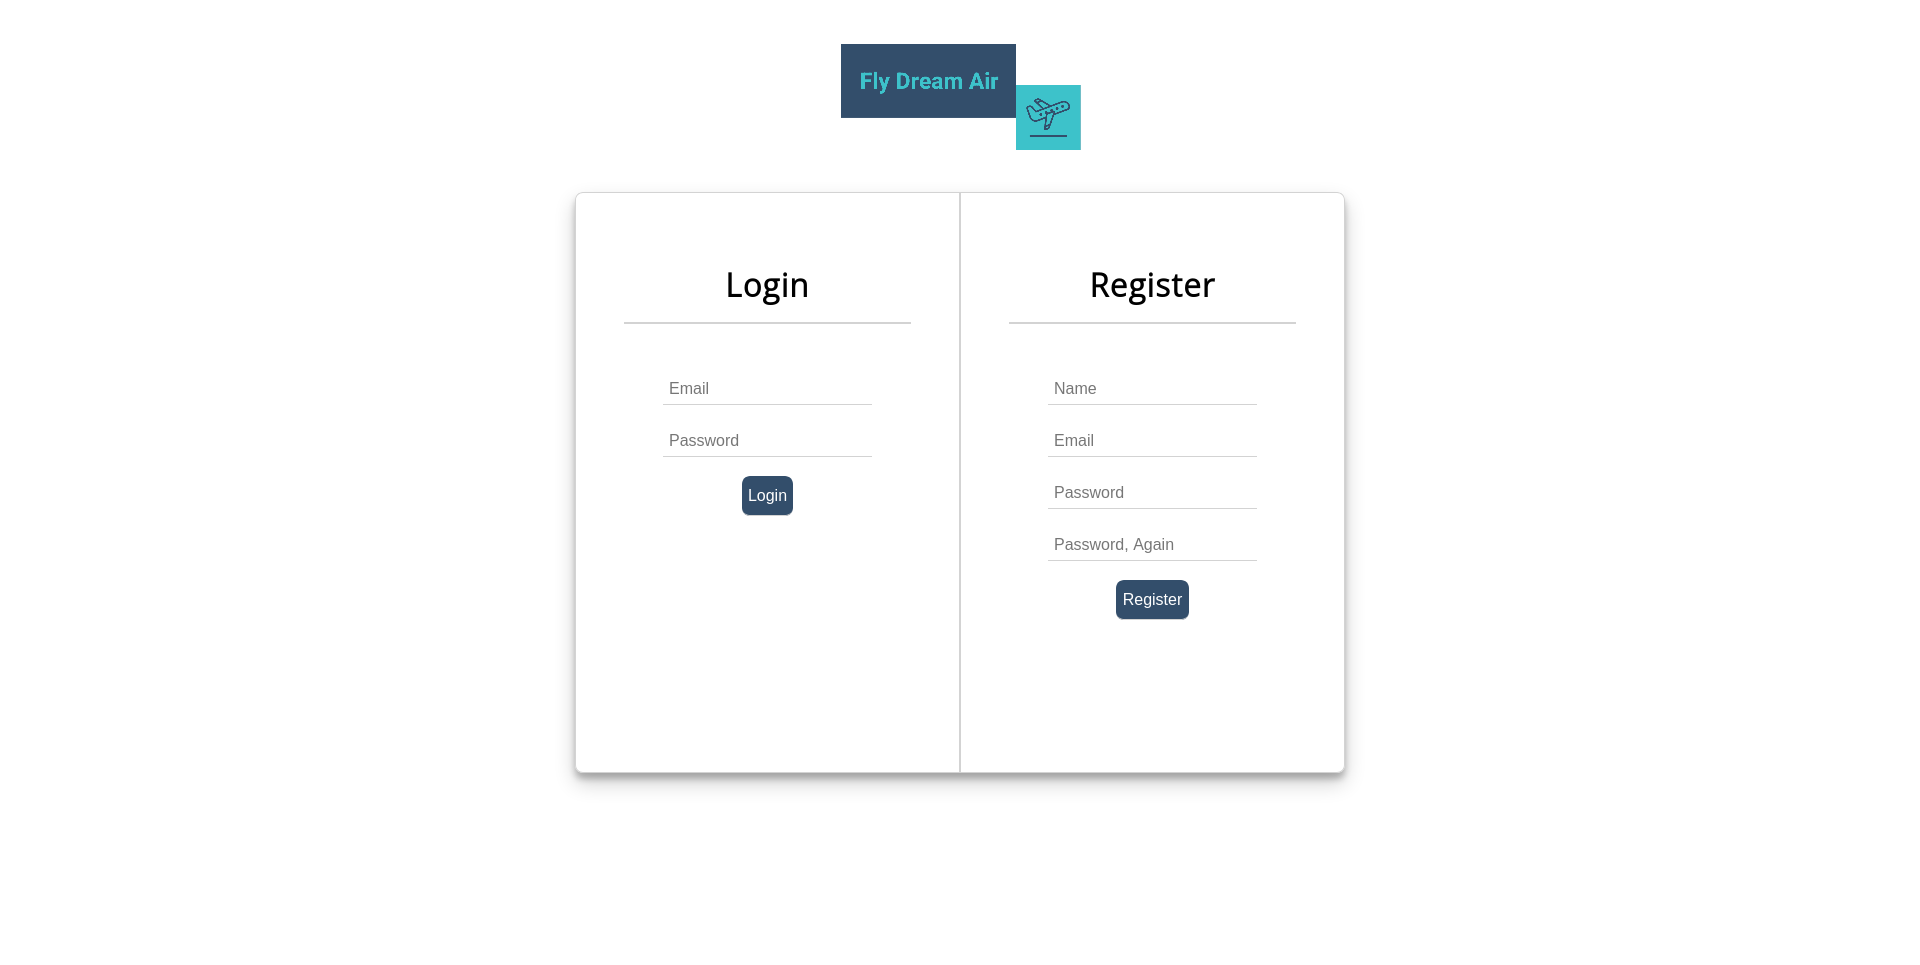
\includegraphics[width=\textwidth]{login}
\end{frame}

\begin{frame}[plain]
  \frametitle{Demo}
  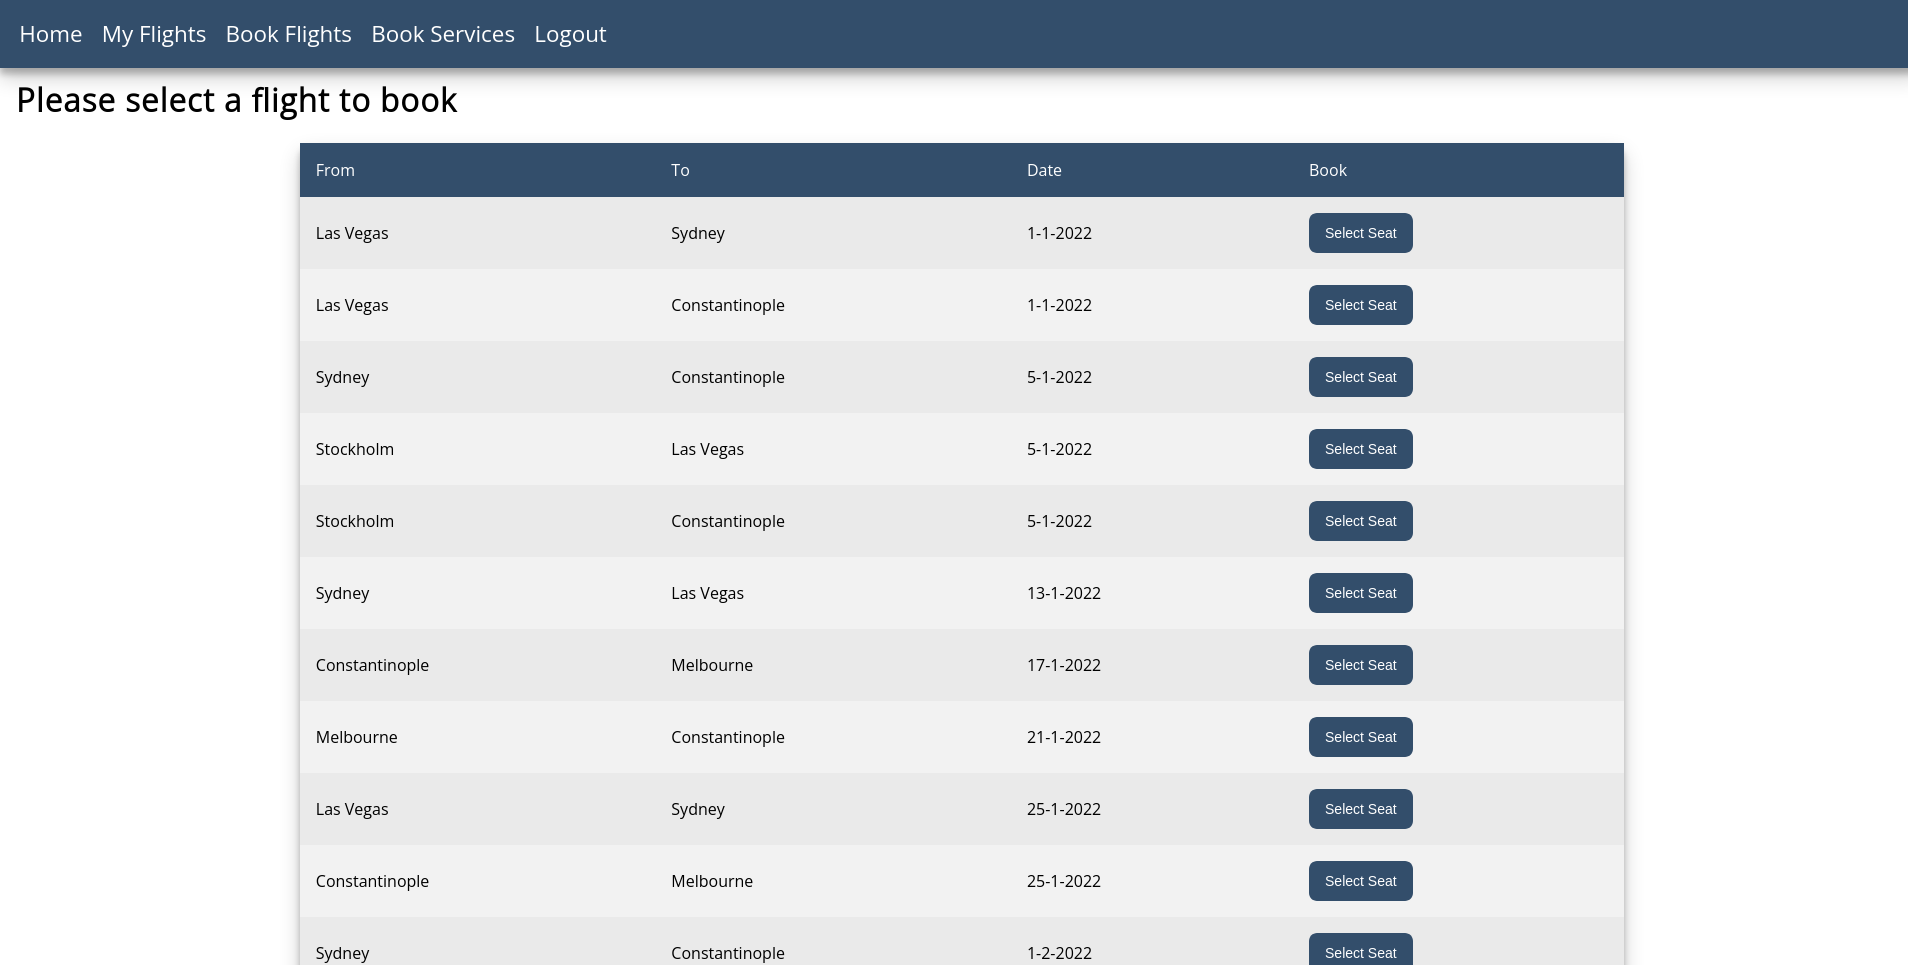
\includegraphics[width=\textwidth]{flights}
\end{frame}

\begin{frame}[plain]
  \frametitle{Demo}
  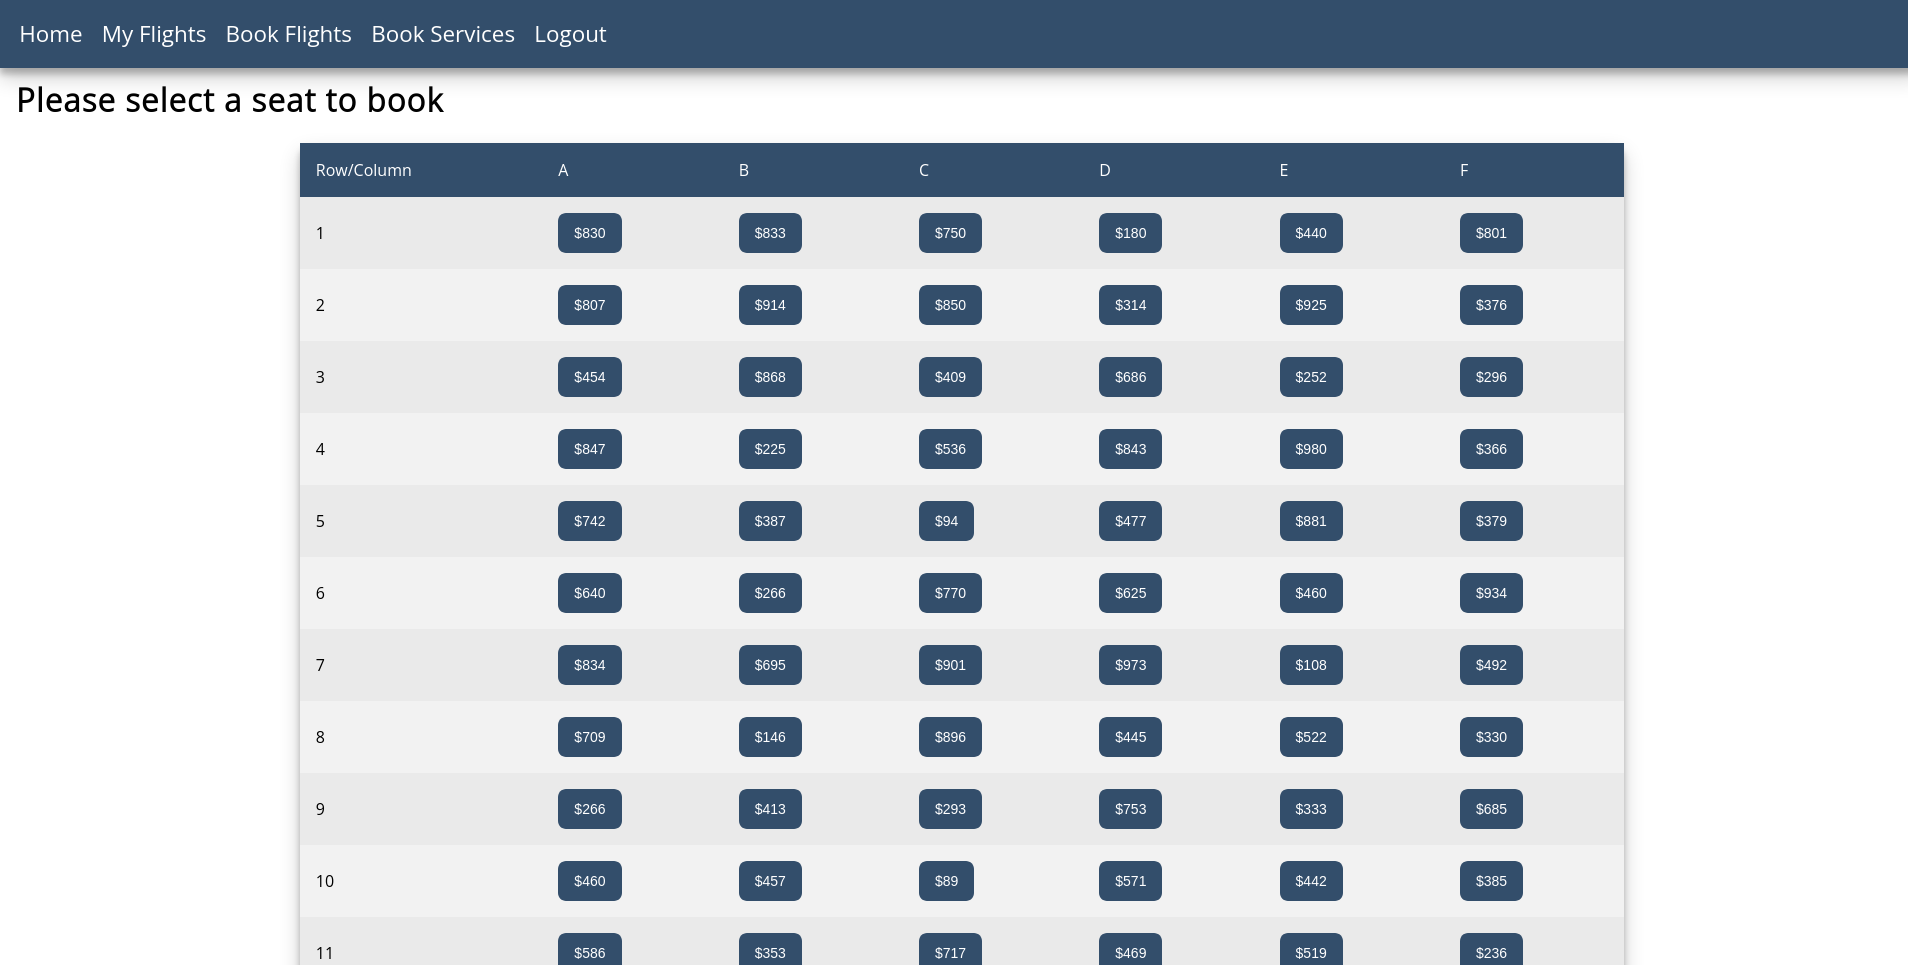
\includegraphics[width=\textwidth]{seat}
\end{frame}

\begin{frame}[plain]
  \frametitle{Demo}
  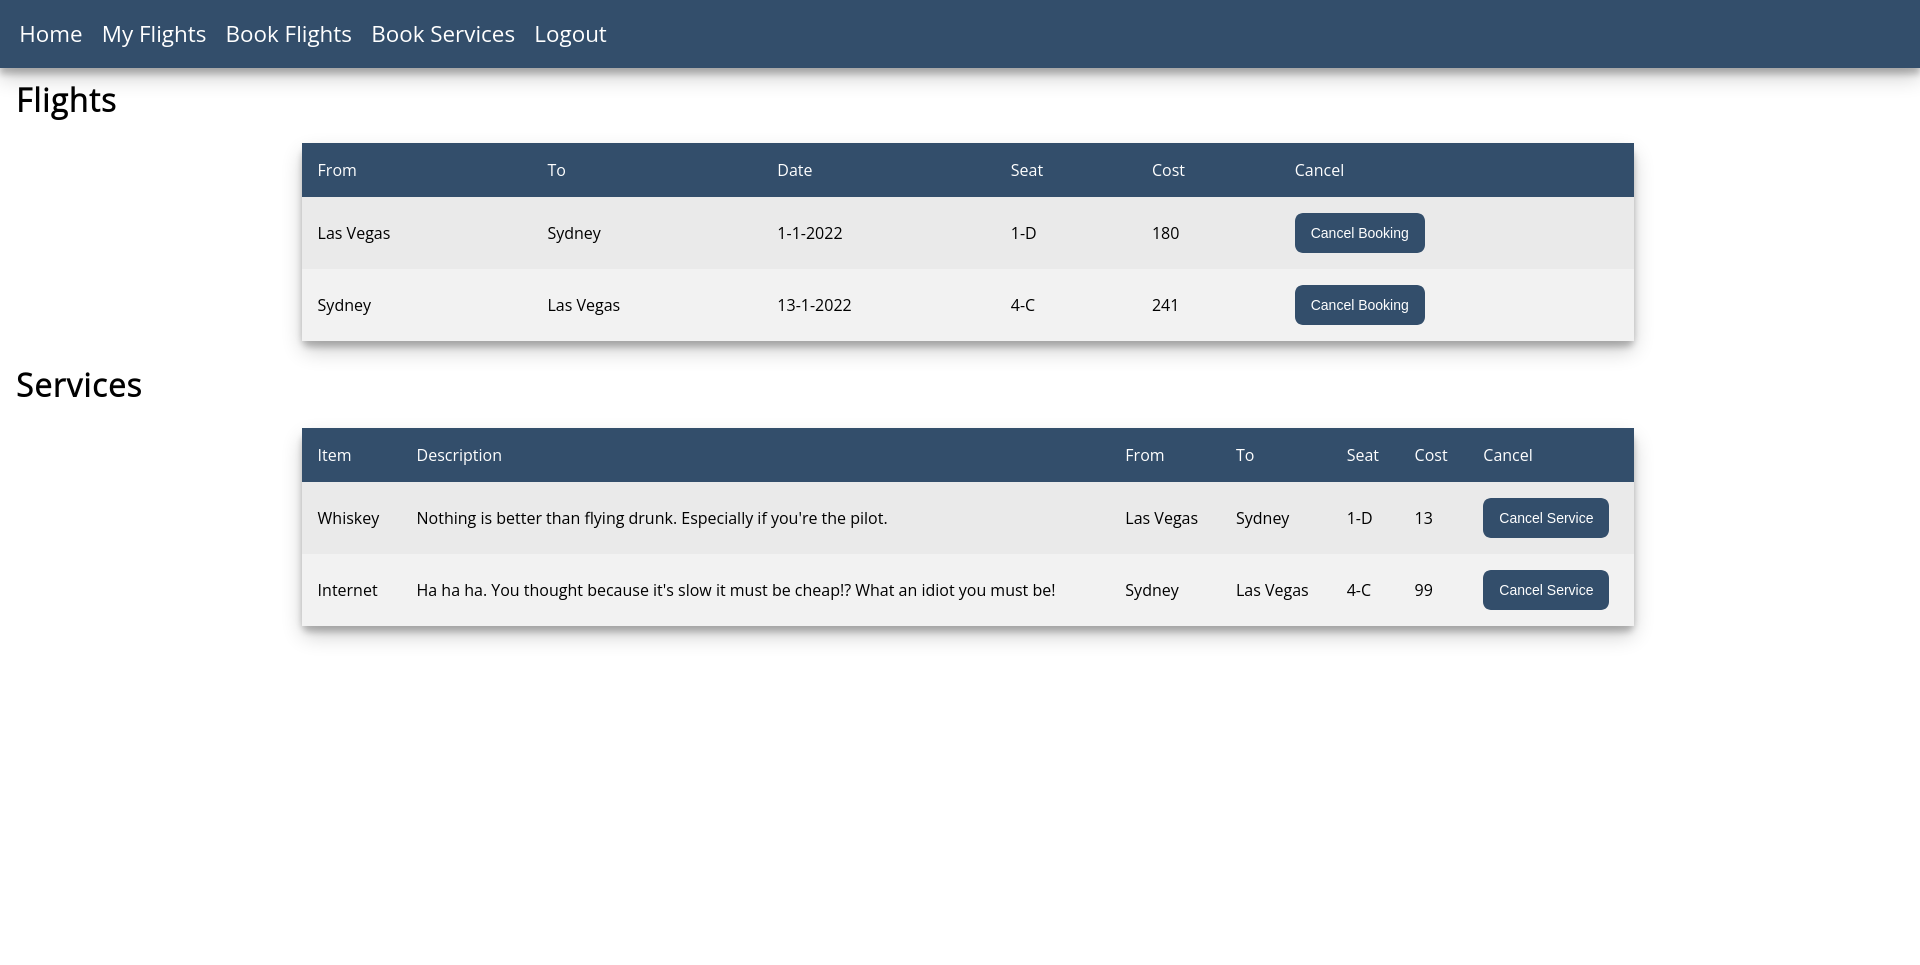
\includegraphics[width=\textwidth]{booked}
\end{frame}

\begin{frame}[plain]
  \frametitle{Questions}
\end{frame}
\end{document}